\section{Fundamental Matrix Estimation}
\label{sec:fundmatrix}

In this section you will explore different methods of estimating the fundamental matrix given a pair of images. In the $\texttt{data/}$ directory, you will find two images (see \autoref{fig:temple_dataset}) from the Middlebury multi-view dataset\footnote{\url{http://vision.middlebury.edu/mview/data/}}, which is used to evaluate the performance of modern 3D reconstruction algorithms.
\begin{figure}[h]
    \centering
    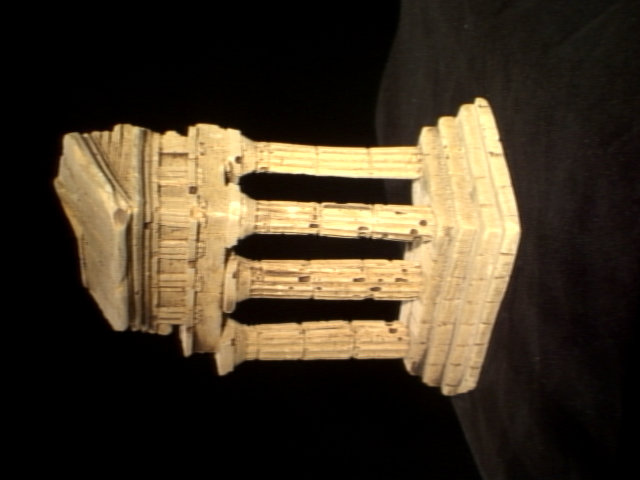
\includegraphics[width=0.35\textwidth]{images/im1.png}\ \
    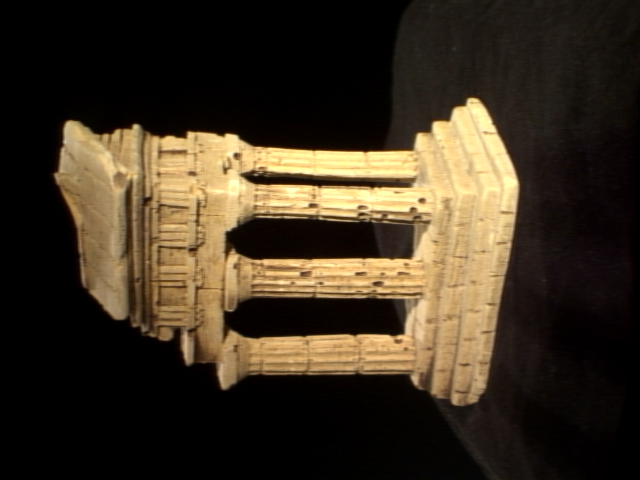
\includegraphics[width=0.35\textwidth]{images/im2.png}
\caption{\texttt{Temple} images for this assignment}
    \label{fig:temple_dataset}
\end{figure}


\subsection{The Eight Point Algorithm}

The 8-point algorithm (discussed in class, and outlined in Section 8.1 of \cite{forsyth2002computer}) is arguably the simplest method for estimating the fundamental matrix. For this section, you can use provided correspondences you can find in \texttt{data/some\_corresp.npz}.


\subparagraph*{Q2.1}\points{10}
\begin{figure}[t]
    \centering
    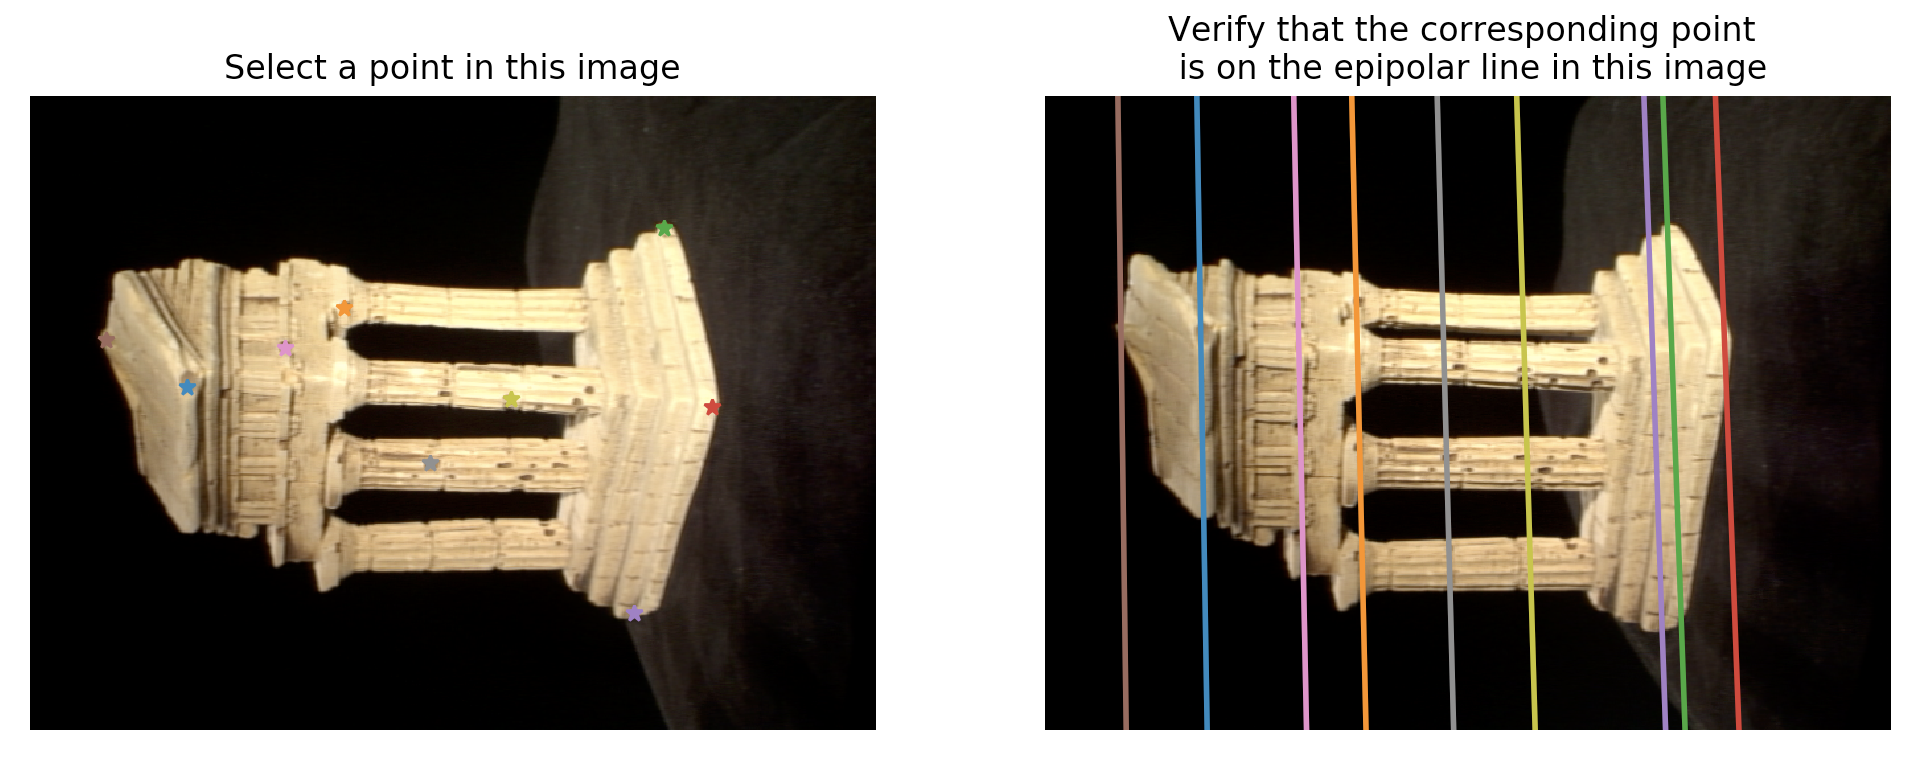
\includegraphics[width=0.8\textwidth]{images/q1_3_epi.png}
    \caption{\texttt{displayEpipolarF} in \texttt{helper.py} creates a GUI for visualizing epipolar lines}
    \label{fig:epigui}
\end{figure}
Finish the function \texttt{eightpoint} in \texttt{q2\_1\_eightpoint.py}. Make sure you follow the signature for this portion of the assignment:
\begin{center}
    \texttt{F = eightpoint(pts1, pts2, M)}
\end{center}
where \texttt{pts1} and \texttt{pts2} are $N \times 2$ matrices corresponding to the $(x,y)$ coordinates of the $N$ points in the first and second image respectively. \texttt{M} is a scale parameter.
\begin{itemize}
    \item You should scale the data as was discussed in class, by dividing each coordinate by $M$ (the maximum of the image's width and height). After computing $\F$, you will have to ``unscale'' the fundamental matrix.
    \\\emph{Hint:} If $\x_{normalized} = \T\x$, then $\F_{unnormalized} = \T^T \F \T$.
    \\You must enforce the singularity condition of $\F$ before unscaling.

    \item You may find it helpful to refine the solution by using local minimization.  This probably won't fix a completely broken solution, but may make a good solution better by locally minimizing a geometric cost function. For this we have provided a helper function \texttt{refineF} in \texttt{helper.py} taking in $\F$ and the two sets of points, which you can call from \texttt{eightpoint} before unscaling \texttt{F}.

    \item Remember that the $x$-coordinate of a point in the image is its column entry, and $y$-coordinate is the row entry. Also note that eight-point is just a figurative name, it just means that you need at least 8 points; your algorithm should use an over-determined system ($N>8$ points).

    \item To visualize the correctness of your estimated $\F$, use the function \texttt{displayEpipolarF} in \texttt{helper.py}, which takes in $\F$, and the two images. This GUI lets you select a point in one of
    the images and visualize the corresponding epipolar line in the other image (\autoref{fig:epigui}).
    
    \item In addition to visualization, we also provide a test code snippet in \texttt{q2\_1\_eightpoint.py} which uses helper function \texttt{calc\_epi\_error} to evaluate the quality of the estimated fundamental matrix. This function calculates the distance between the estimated epipolar line and the corresponding points. For the eight point algorithm, the error should on average be $< 1$. 

\end{itemize}

\deliver{
\textbf{Output:} Save your matrix $\F$ and scale \texttt{M} to the file \texttt{q2\_1.npz}.\\
\textbf{In your write-up:} 
\begin{itemize}
    \item Write your recovered $\F$
    \item Include an image of some example output of \texttt{displayEpipolarF}
    \item Include the code snippet of \texttt{eightpoint} function
\end{itemize}
}

\begin{your_solution}[title=Q2.1,height=23.2cm,width=\linewidth]
As in the output: $./q2\_1.npz$, the recovered F is: 
\newline

$\begin{pmatrix}
	-2.19293792e^{-07} &  2.95926413e^{-05} & -2.51886251e^{-01} \\
	1.28064423e^{-05}  & -6.64493522e^{-07} &  2.63771761e^{-03} \\
	2.42228993e^{-01}  & -6.82585388e^{-03} &  1.00000000e^{+00}
\end{pmatrix}$
\newline

Besides, M = 640.
\newline
The following \autoref{fig:Q2_1_result} shows the result of the Eight Point Algorithm:
\newline
\begin{minipage}{1\linewidth}
	\centering
	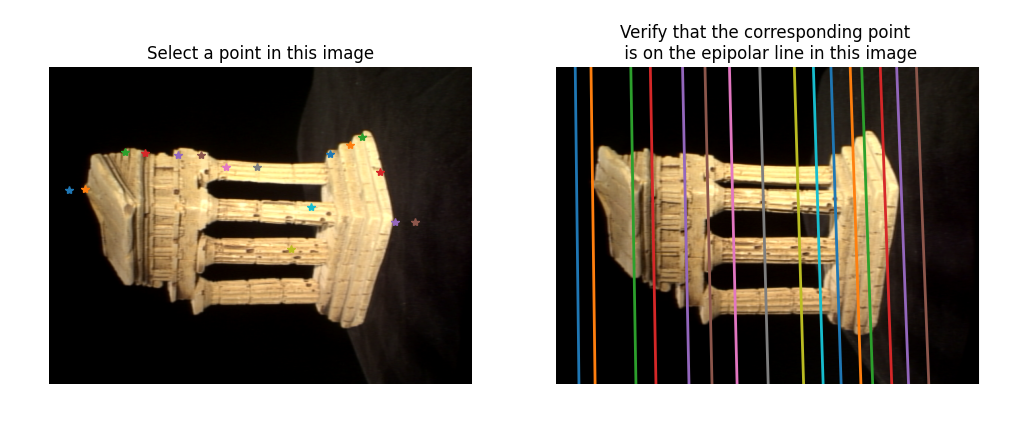
\includegraphics[width=1\linewidth, height=0.39\columnwidth]{../Q2_1_result.png}
	\refstepcounter{figure}  % Increment the figure counter
	\textbf{Figure \ref{fig:Q2_1_result}:} Result of the Eight Point Algorithm  % Manually add a caption/title
	\label{fig:Q2_1_result}         % Label for referencing	
\end{minipage}
\newline

The following \autoref{fig:first_image} and \autoref{fig:second_image} show the code snippet of the Eight Point Algorithm in q2\_1\_eightpoint.py:
\newline
\begin{minipage}{0.48\linewidth}
	\centering
	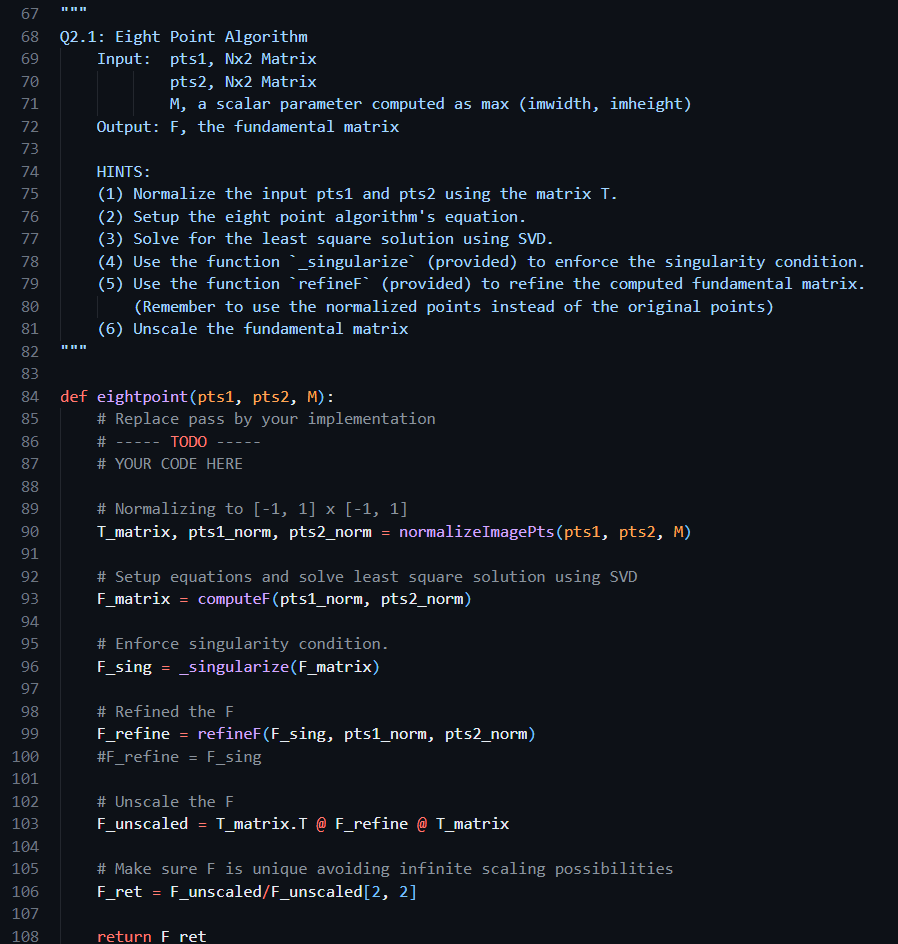
\includegraphics[width=\linewidth]{../Q2_1_cns1.png}
	\refstepcounter{figure}  % Increment the figure counter
    \textbf{Figure \ref{fig:first_image}:} First Code Snippet  % Manually add a caption/title
	\label{fig:first_image}         % Label for referencing	
\end{minipage}
\hfill
\begin{minipage}{0.48\linewidth}
	\centering
	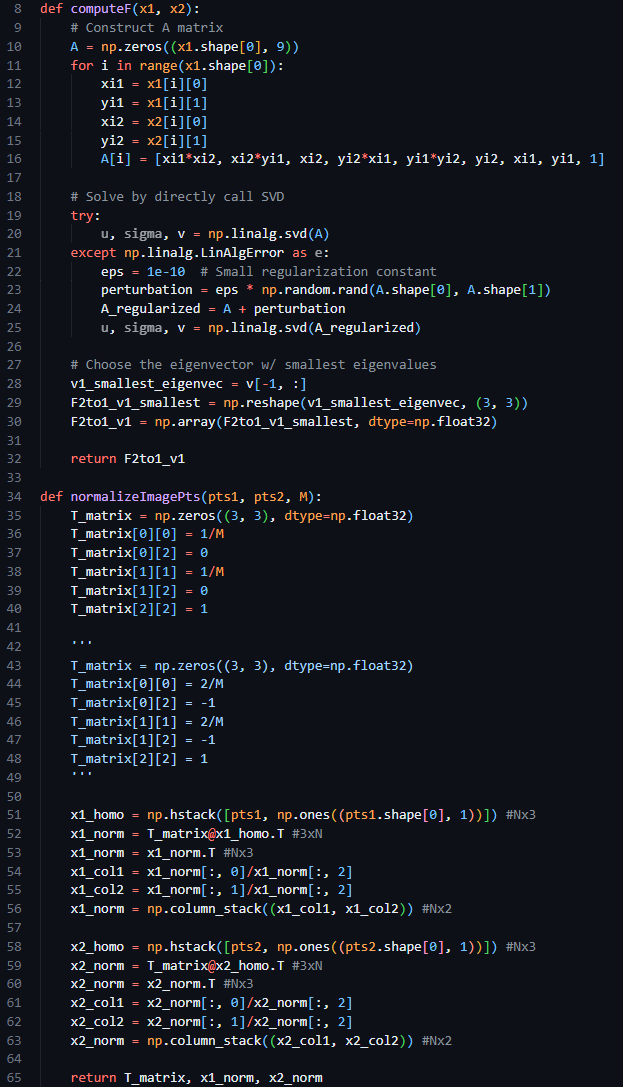
\includegraphics[width=\linewidth, height=1.43\columnwidth]{../Q2_1_cns2.png}
	\refstepcounter{figure}  % Increment the figure counter
	\textbf{Figure \ref{fig:second_image}:} Second Code Snippet  % Manually add a caption/title
	\label{fig:second_image}         % Label for referencing
\end{minipage}


\end{your_solution}

\subsection{The Seven Point Algorithm (Extra Credit)}
% The Seven-Point Algorithm

Since the fundamental matrix only has seven degrees of freedom, it is possible to calculate $\textbf{F}$ using only seven-point correspondences. This requires solving a polynomial equation.  In this section, you will implement the seven-point algorithm  (outlined in this \href{https://imkaywu.github.io/blog/2017/06/fundamental-matrix/}{\textcolor{blue}{post}}). 

\subparagraph*{Q2.2} \points{Extra Credit - 15}
Finish the function \texttt{sevenpoint} in \texttt{q2\_2\_sevenpoint.py}. Make sure you follow the signature for this portion of the assignment:
\begin{center}
    \texttt{Farray = sevenpoint(pts1, pts2, M)}
\end{center}
where pts1 and pts2 are $7 \times 2$ matrices containing the correspondences and \texttt{M} is the normalizer (use the maximum of the image's height and width), and \texttt{Farray} is a list array of length either 1 or 3 containing Fundamental matrix/matrices. Use \texttt{M} to normalize the point values between $[0,1]$ and remember to ``unnormalize" your computed $\textbf{F}$ afterward.

Manually select $7$ points from the provided point in \texttt{data/some\_corresp.npz}, and use these points to recover a fundamental matrix $\textbf{F}$. Use \texttt{calc\_epi\_error} in \texttt{helper.py} to calculate the error to pick the best one, and use \texttt{displayEpipolarF} to visualize and verify the solution.

\deliver{
\textbf{Output:} Save your matrix $\F$ and scale \texttt{M} to the file \texttt{q2\_2.npz}.\\
\textbf{In your write-up: }
\begin{itemize}
    \item Write your recovered $\textbf{F}$ 
    \item Include an image of some example output of \texttt{displayEpipolarF}
    \item Include the code snippet of \texttt{sevenpoint} function
\end{itemize}
}

\begin{your_solution}[title=Q2.2,height=21.5cm,width=\linewidth]
As in the output: $./q2\_2.npz$, the recovered F is: 
\newline

$\begin{pmatrix}
8.10457547e^{-07} &  8.90918216e^{-06} & -2.01028479e^{-01} \\
2.63329923e^{-05} & -6.00542314e^{-07} &  6.97427247e^{-04} \\
1.92182103e^{-01} & -4.20123320e^{-03} &  1.00000000e^{+00}
\end{pmatrix}$
\newline

Besides, M = 640.
\newline
The following \autoref{fig:Q2_2_result} shows the result of the Eight Point Algorithm:
\newline
\begin{minipage}{1\linewidth}
	\centering
	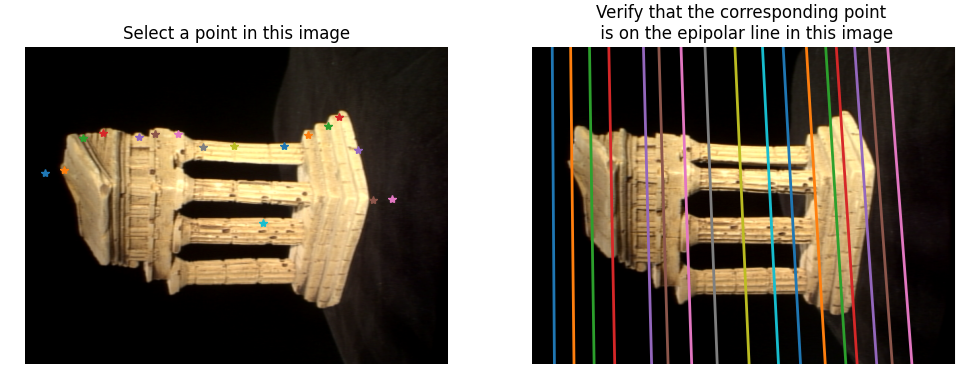
\includegraphics[width=\linewidth]{../Q2_2_result.png}
	\refstepcounter{figure}  % Increment the figure counter
	\textbf{Figure \ref{fig:Q2_2_result}:} Result of the Seven Point Algorithm  % Manually add a caption/title
	\label{fig:Q2_2_result}         % Label for referencing	
\end{minipage}
\newline

The following \autoref{fig:Q2_2_cns1}, \autoref{fig:Q2_2_cns2}, \autoref{fig:Q2_2_cns3} and \autoref{fig:Q2_2_cns4} show the code snippet of the Seven Point Algorithm in q2\_2\_sevenpoint.py:
\newline


\begin{minipage}{0.48\linewidth}
	\centering
	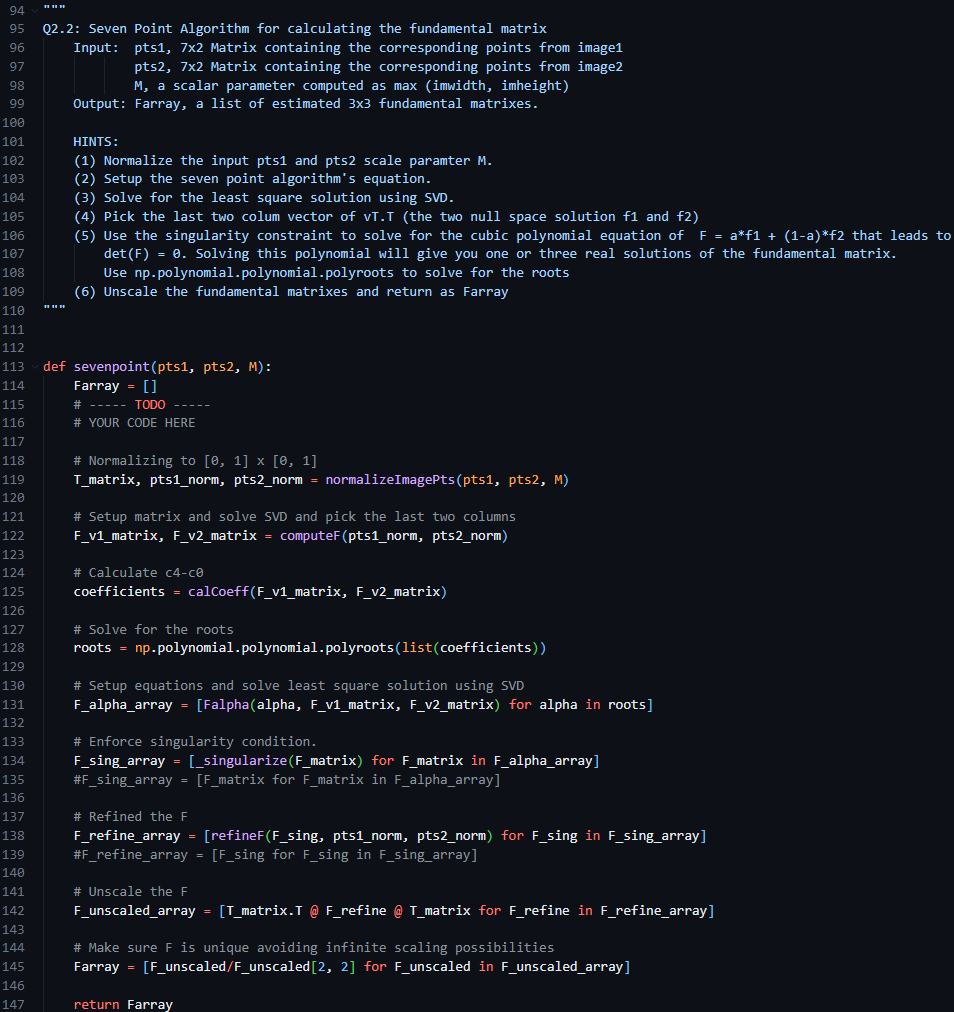
\includegraphics[width=\linewidth]{../Q2_2_cns1.png}
	\refstepcounter{figure}  % Increment the figure counter
	\textbf{Figure \ref{fig:Q2_2_cns1}:} First Code Snippet  % Manually add a caption/title
	\label{fig:Q2_2_cns1}         % Label for referencing	
\end{minipage}
\hfill
\begin{minipage}{0.48\linewidth}
	\centering
	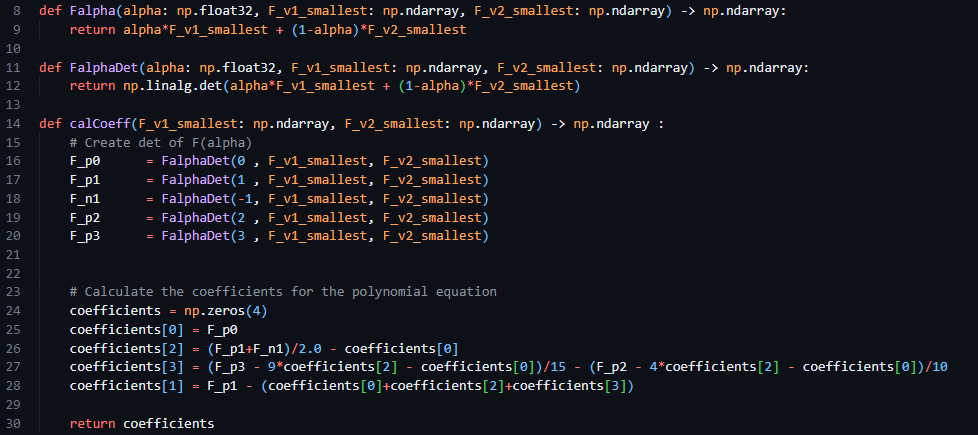
\includegraphics[width=\linewidth]{../Q2_2_cns2.png}
	\refstepcounter{figure}  % Increment the figure counter
	\textbf{Figure \ref{fig:Q2_2_cns2}:} Second Code Snippet  % Manually add a caption/title
	\label{fig:Q2_2_cns2}         % Label for referencing
\end{minipage}	
\newline
\end{your_solution}
\newpage
\begin{your_solution}[title=Q2.2 continued,height=10.0cm,width=\linewidth]
\begin{minipage}{0.48\linewidth}
	\centering
	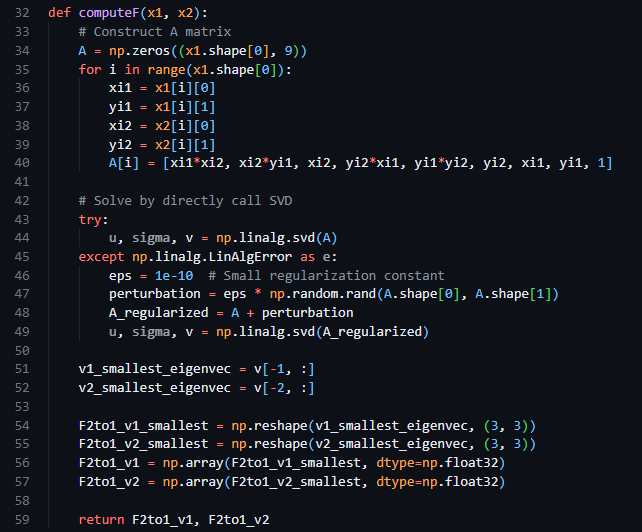
\includegraphics[width=\linewidth]{../Q2_2_cns3.png}
	\refstepcounter{figure}  % Increment the figure counter
	\textbf{Figure \ref{fig:Q2_2_cns3}:} Third Code Snippet  % Manually add a caption/title
	\label{fig:Q2_2_cns3}         % Label for referencing	
\end{minipage}
\hfill
\begin{minipage}{0.48\linewidth}
	\centering
	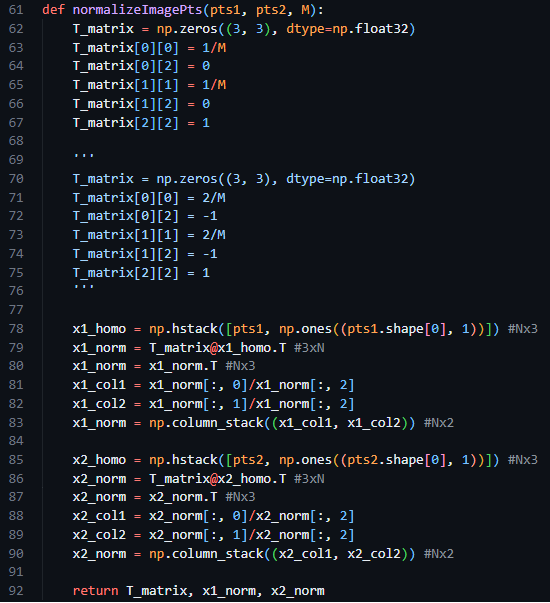
\includegraphics[width=\linewidth]{../Q2_2_cns4.png}
	\refstepcounter{figure}  % Increment the figure counter
	\textbf{Figure \ref{fig:Q2_2_cns4}:} Fourth Code Snippet  % Manually add a caption/title
	\label{fig:Q2_2_cns4}         % Label for referencing
\end{minipage}
\end{your_solution}
